\renewcommand{\familydefault}{\sfdefault}
\documentclass{scrartcl}
\usepackage{amsmath}
\usepackage[utf8]{inputenc}
\usepackage{natbib}
\usepackage{graphicx}
\usepackage{tikz}
\usepackage{float}
\usepackage{bm}
\usepackage{hyperref}
\usepackage{tcolorbox}
\interfootnotelinepenalty=10000000
\newtcolorbox{mybox}{colback=gray!30,
boxrule=0pt,arc=0pt,boxsep=2pt,left=2pt,right=2pt,leftrule=1pt}

\begin{document}
\title{Ring on a rod}
\author{Bob the legend}
\date{\today}
\setlength\parindent{0pt}


\maketitle

\section{Steady state motion (threadless rod) with no slip}
\subsection{Overview of theory}
Just referred to a part in Morin. Basically the goal of this theory is to be able to find the terminal velocity (translational and angular) of the ring.

\begin{enumerate}
    \item Calculate the principal moments of the ring
    \item Calculate angular momentum
    \item Calculate $\frac{d\mathbf{L}}{dt}$
    \item Calculate torque
    \item Equate torque  to $\frac{d\mathbf{L}}{dt}$
\end{enumerate}

Apparently, the equation
\begin{equation}
    \mathbf{\tau}=\frac{d\mathbf{L}}{dt}
\end{equation}
works in a non inertial frame as well (rotating frame) if angular momentum and torque are both calculated with respect to the object's centre of mass (so I think we should do that).

See below for the 2 stack exchange posts I found regarding this:
\begin{mybox}
    \href{https://physics.stackexchange.com/questions/559157/how-to-find-origin-for-angular-momentum?rq=1}{how-to-find-origin-for-angular-momentum?}
    \newline
    \href{https://physics.stackexchange.com/questions/176205/angular-momentum-torque-relationship-in-a-rotating-frame}{angular-momentum-torque-relationship-in-a-rotating-frame}
\end{mybox}

So in this case, the ring's motion can be decomposed into rotation about its COM ($\mathbf{\Omega}$) + rotation of COM about the centre of the rod ($\boldsymbol{\omega}$). It is relatively simple to analyse the the motion of the ring in the rotating frame (the COM frame).



\subsection{Geometry}
The principal axes are defined as any 2 orthogonal axes ($y$ and $z$) parallel to the ring, along with 1 axis perpendicular to the ring ($x$). The positive z axis points out of the page. The pricipal moments (relative to the object's centre of mass) are
\begin{equation}
    \mathbf{I_1}=\Bigg(\frac{1}{12}m(3(R_1^2+R_2^2)+d^2),
    \frac{1}{2}m(R_1^2+R_2^2),
    \frac{1}{12}m(3(R_1^2+R_2^2)+d^2)\Bigg)
\end{equation}
\begin{figure}[h]
    \centering
    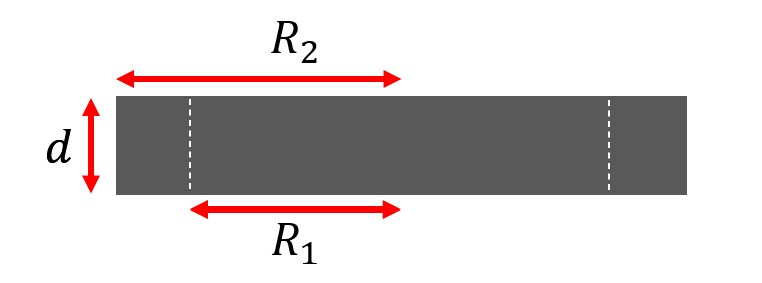
\includegraphics[scale=0.5]{diagram2.jpg}
    \caption{Geometry of the ring}
    \label{1}
\end{figure}

\subsection{Angular momentum}
\begin{figure}[h]
    \centering
    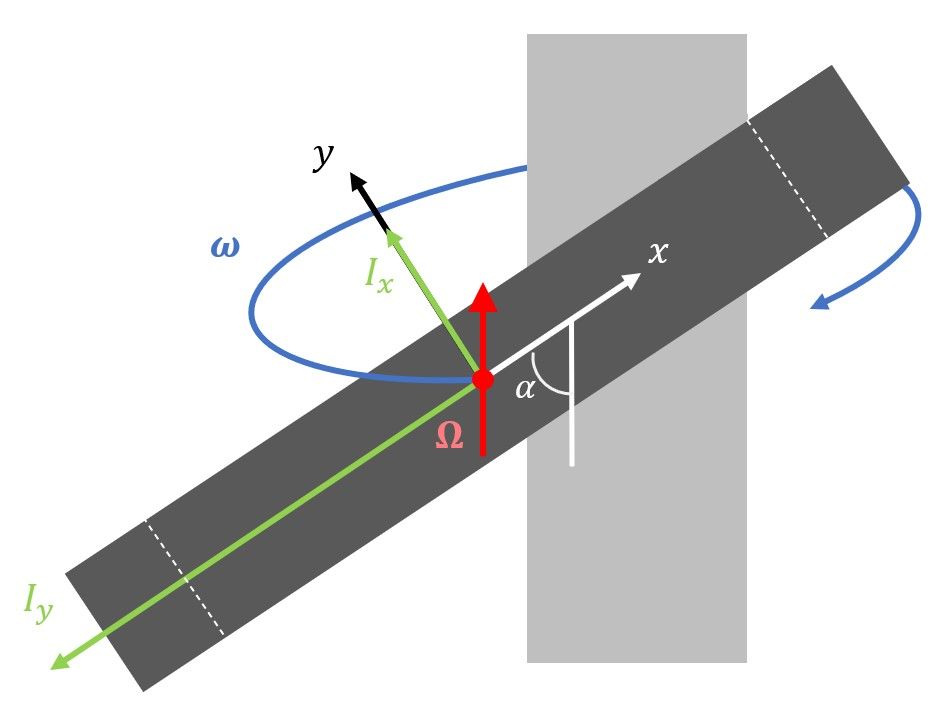
\includegraphics[scale=0.4]{diagram1.jpg}
    \caption{Coordinate system (in rotating frame), $x_3$ and $I_3$ are pointing out of the page}
    \label{<2>}
\end{figure}

In the frame that rotates together with the ring's COM, the $\mathbf{\Omega}$ vector points vertically upwards. In the basis of the principal axes of the rings ($x$,$y$,$z$):

\begin{equation}
    \mathbf{\Omega}=(\Omega\cos\alpha,\Omega\sin\alpha,0)
\end{equation}

Hence, the angular momentum, $\mathbf{L}$ of the ring in this frame is thus:
\begin{equation}
    \begin{aligned}
        L & =(I_x\Omega_x,I_y\Omega_y,I_z\Omega_z)       \\
          & =(I_x\Omega\cos\alpha,I_y\Omega\sin\alpha,0)
    \end{aligned}
\end{equation}
To find the rate of change of angular momentum, we use the following relationship:
\begin{equation}
    \begin{aligned}
        \frac{d\mathbf{L}}{dt} & =\mathbf{\Omega}\times\mathbf{L}                                                   \\
                               & =(L_y\Omega_z-L_z\Omega_y)\mathbf{\hat{x}}+
        (L_z\Omega_x-L_x\Omega_z)\mathbf{\hat{y}}+
        (L_x\Omega_y-L_y\Omega_x)\mathbf{\hat{z}}                                                                   \\
                               & = (L_x\Omega\sin\alpha-L_y\Omega\cos\alpha)\mathbf{\hat{z}}                        \\
                               & =(I_x\Omega^2\sin\alpha\cos\alpha-I_y\Omega^2\sin\alpha\cos\alpha)\mathbf{\hat{z}}
    \end{aligned}
\end{equation}
Taking the magnitude:
\begin{equation}
    \left| \frac{d\mathbf{L}}{dt} \right|=(I_y-I_x)\Omega^2\sin\alpha\cos\alpha\mathbf{\hat{z}}
\end{equation}
pointing into the page.

\subsection{no slip constraint to relate $\Omega$ with $\omega$}

We still need to introduce a no-slip constraint to relate $\Omega$ with $\omega$. I am not so sure about this but maybe it is
\begin{equation}
    \begin{aligned}
        \omega r & =  \Omega_y R_1         \\
                 & = \Omega R_1 \sin\alpha
    \end{aligned}
\end{equation}

\subsection{Terminal velocity}
If we observe the motion of the ring in its COM frame, we will realise that the contact point will move downwards by $2R_1\cos\alpha$ every half round (assuming no slip).

\begin{figure}[htbp]
    \centering
    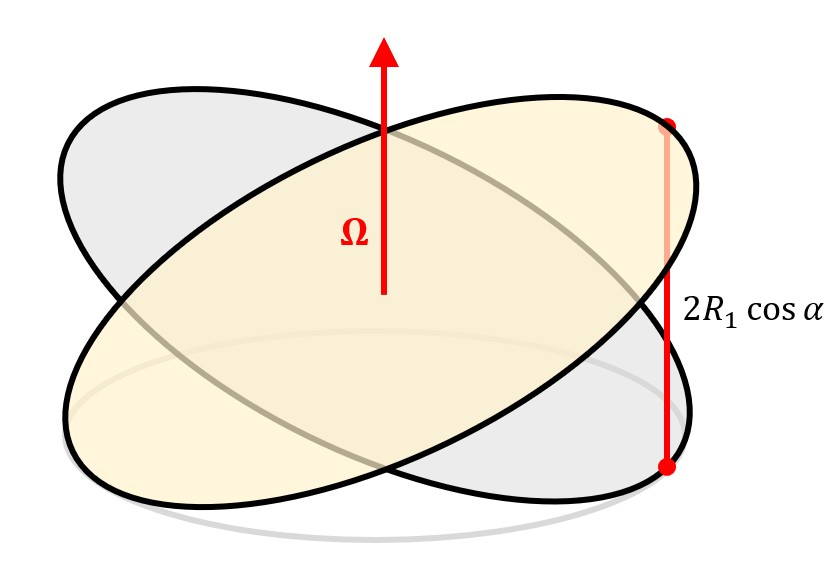
\includegraphics[scale=0.5]{diagram5.jpg}
    \caption{Motion of contact point}
    \label{5}
\end{figure}
This means that the path traced out by the contact point is in fact helical, described by the following equation:
\begin{equation}
    S=(r \cos t)\mathbf{\hat{x}} +(r \sin t)\mathbf{\hat{y}}+ct\mathbf{\hat{z}}
\end{equation}
where $c=(2R_1\sin\alpha )t/\pi$.
The helix's radius of curvature (I realised this may not be so useful but will just leave it here) is then given by
\begin{equation}
    R_c= \frac{r^2+c^2}{r}
\end{equation}


The terminal velocity of the ring can then be calculated as \begin{equation}
    v= \frac{d}{t}= \frac{2\Omega R_1 \cos\alpha}{\pi}
\end{equation}

\subsection{Torque}
The only 2 forces that exert torque about the COM are friction and the horizontal normal force (for non threaded rod). Since we are analysing the \textbf{non-slip steady state motion} of the ring, balancing forces in the vertical and radial direction gives us:
\begin{equation}
    \begin{cases}
        f=mg \\
        N=m(R_1\sin\alpha)\omega^2
    \end{cases}
\end{equation} and  must be true

\begin{figure}[h]
    \centering
    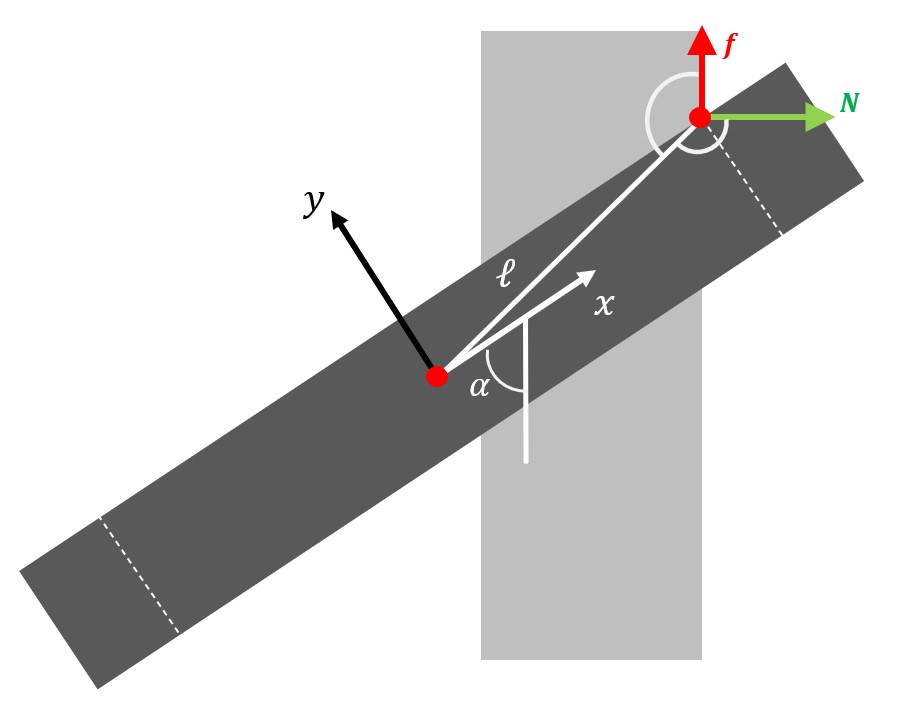
\includegraphics[scale=0.4]{diagram4.jpg}
    \caption{Free body diagram I guess}
    \label{4}
\end{figure}

We can then calculate the torque by these forces about COM as such:
\begin{equation}
    \left|\tau\right| =N\ell\cos(\alpha-\beta)- f\ell\sin(\alpha-\beta)
\end{equation}
where $\ell=\sqrt{R_1^2+(d/2)^2}$ and $\beta=\arctan(d/2R_1)$  and it points into the page as well.

Equating torque to the rate of change of angular momentum which we calculated just now:
\begin{equation}
    N\ell\cos(\alpha-\beta)- f\ell\sin(\alpha-\beta)= (I_y-I_x)\Omega^2 \sin\alpha\cos\alpha
\end{equation}

Substituting in the expression for $f$ and $N$, as well as the non slip condition, we get

\begin{equation}
    \boxed{
        \Omega^2=\frac{mg\ell\sin(\alpha-\beta)r^2}{mR_1^2R_2\ell\sin^3\alpha\cos(\alpha-\beta)-(I_y-I_x)r^2\sin\alpha\cos\alpha}}
\end{equation}

\section{References}
\href{https://physics.stackexchange.com/questions/686439/physics-of-mad-tea-party}{https://physics.stackexchange.com/questions/686439/physics-of-mad-tea-party}
\newline
\href{https://amesweb.info/inertia/hollow-cylinder-moment-of-inertia.aspx}{https://amesweb.info/inertia/hollow-cylinder-moment-of-inertia.aspx}

\section{Another theory which I realised was definitely wrong so can ignore from here onwards}

I think this whole theory is \textbf{extremely questionable} because
\begin{itemize}
    \item I am ignoring friction, which is a key reason why the ring will reach a terminal velocity. (energy gained from GPE dissipated through friction, so KE and RKE remains the same)
    \item The ring's motion has been decomposed into its rotation about COM and the rotation of COM about the rod is slightly questionable.
    \item The way I calculated torque from angular momentum is very questionable. Normally, when we visualise the angular momentum vector, it should have an origin (e.g. angular momentum of pendulum points out from the pivot). But in this case, I don't think it is possible to find such an origin. So I don't know whether I should calculate torque about contact point? COM? Or some other points. I asked around online and the people said that angular momentum is not in fact an vector; but it can be put \textbf{in bijection with a vector}.
          \begin{mybox}
              Each axis has its own angular momentum. The angular momentum has magnitude, and the axis has direction, so this combination of magnitude and direction looks like a vector, but it isn't really, and it doesn't have an origin in physical space. It makes sense to depict it as having its origin on the corresponding axis, and often the axis being considered goes through the center of mass, making the center of mass a natural choice for the origin, but the choice to depict its origin there doesn't really correspond to anything physical.

              Even angular momentum "vectors" with the same "origin" can't be added like normal vectors if they have different axes (you get things like precession that wouldn't appear if they were truly vectors), and it's even more complicated to combine angular momenta from different axes.
          \end{mybox}
          so uhm this thing is kinda confusing.
\end{itemize}

\subsection{Overview of theory}
Just referred to a part in Morin. Basically the goal of this theory is to be able to find the terminal frequency of motion of the ring about the rod.

\begin{enumerate}
    \item Calculate the principal moments of the ring
    \item Calculate angular momentum
    \item Calculate $\frac{d\mathbf{L}}{dt}$
    \item Calculate torque
    \item Equate torque  to $\frac{d\mathbf{L}}{dt}$
\end{enumerate}

Let's visualise the motion as a rotation of the ring about its centre of mass ($\mathbf{\Omega}$), and the rotation of the centre of mass about the centre of the rod ($\boldsymbol{\omega}$), as illustrated in the figure below.

\begin{figure}[h]
    \centering
    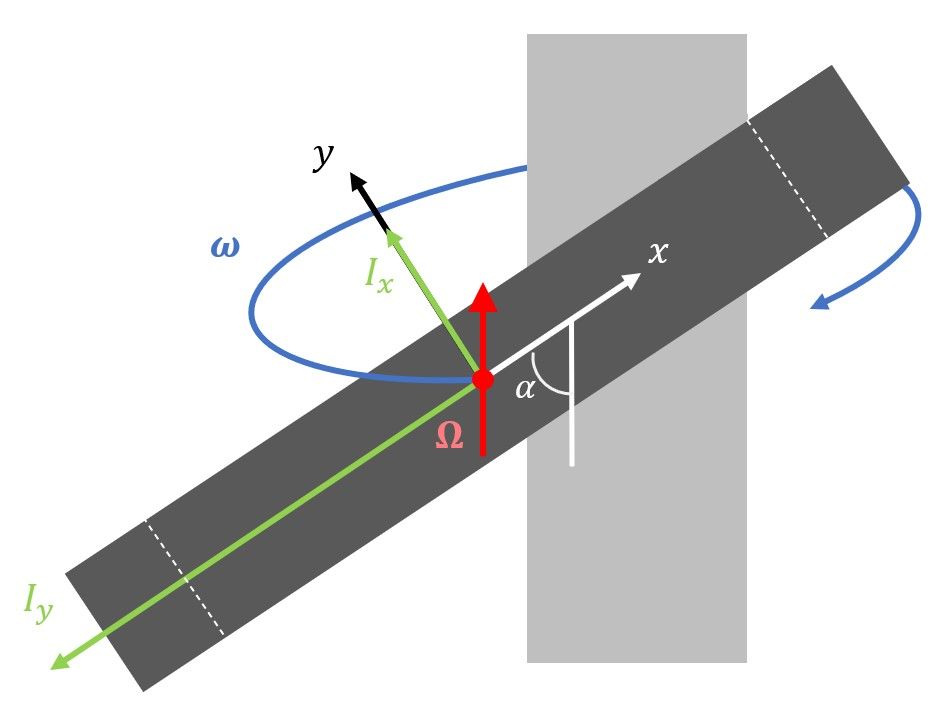
\includegraphics[scale=0.4]{diagram1.jpg}
    \caption{Coordinate system (in rotating frame), $x_3$ and $I_3$ are pointing out of the page}
    \label{2}

\end{figure}

\subsection{Moment of inertia}
\begin{figure}[h]
    \centering
    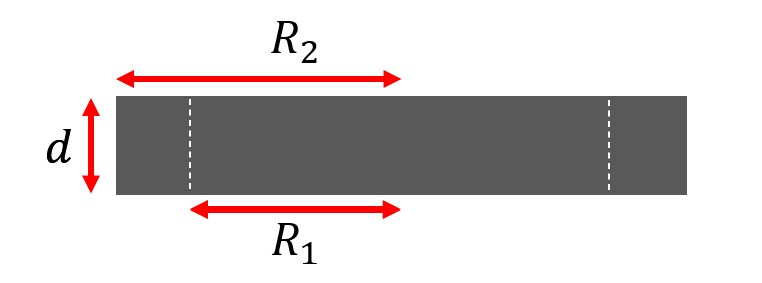
\includegraphics[scale=0.5]{diagram2.jpg}
    \caption{Geometry of the ring}
    \label{1}
\end{figure}

The principal axes are any 2 orthogonal axes ($y$ and $z$) parallel to the ring, along with 1 axis perpendicular to the ring ($x$). The positive z axis points out of the page. The priciple moments (relative to the object's centre of mass) are
\begin{equation}
    \mathbf{I_1}=\Bigg(\frac{1}{12}m(3(R_1^2+R_2^2)+d^2),
    \frac{1}{2}m(R_1^2+R_2^2),
    \frac{1}{12}m(3(R_1^2+R_2^2)+d^2)\Bigg)
\end{equation}
The moments (relative to the centre of the rod using parallel axis theorem) are
\begin{equation}
    \begin{aligned}
        \mathbf{I_2}=\Bigg(\frac{1}{12}m(3(R_1^2+R_2^2)+d^2)+m(R_1\sin\alpha-r)^2 \cos^2\alpha, \\
        \frac{1}{2}m(R_1^2+R_2^2)+m(R_1\sin\alpha-r)^2 \sin^2\alpha,                            \\
        \frac{1}{12}m(3(R_1^2+R_2^2)+d^2)+m(R_1\sin\alpha-r)^2 \cos^2\alpha\Bigg)
    \end{aligned}
\end{equation}

In the frame that rotates together with the ring's COM, the $\mathbf{\Omega}$ vector points vertically upwards. In the basis of the principal axes of the rings ($x$,$y$,$z$):

\begin{equation}
    \mathbf{\Omega}=(\Omega\cos\alpha,\Omega\sin\alpha,0)
\end{equation}
The same applies for $\boldsymbol{\omega}$.

\subsection{Angular momentum}
The angular momentum in the lab frame can be calculated by adding the "spin angular momentum" (angular momentum ring about its COM) to the orbital angular momentum (angular momentum due to rotation of COM about centre of rod).The total angular momentum in the lab frame is thus:

\begin{equation}
    \sum \mathbf{L}=\mathbf{I_1}\boldsymbol{\Omega} + \mathbf{I_2}\boldsymbol{\omega}
\end{equation}

The spin angular momentum is:
\begin{equation}
    L_s= (I_{1,x}\Omega \cos\alpha ,I_{1,y}\Omega \sin\alpha,0)
\end{equation}
The orbital angular momentum is:
\begin{equation}
    L_o= (I_{2,x}\omega \cos\alpha ,I_{2,y}\omega \sin\alpha,0)
\end{equation}

Adding up the 2 components gives us \footnote{This part is very questionable.}:
\begin{equation}
    L=((I_{1,x}\Omega +I_{2,x}\omega)\cos\alpha,(I_{1,y}\Omega +I_{2,y}\omega)\sin\alpha,0)
\end{equation}

\subsection{Torque}
The final angular momentum in the lab frame (labelled as $L$) will precess about the vertical axis (dotted line) due to torque by gravity (about contact point??? yea this is really questionable, since the "origin" of the angular momentum vector is unknown, I have no idea about which point I should calculate torque) \footnote{In most diagrams, if an object is rotating about the contact point (maybe a falling stick with one end pivoted to the floor), $\tau_g$ and $L$ vectors will both be drawn as arrows pointing away from the pivot.}

I will explicitly calculate the horizontal component of the angular momentum.

\begin{figure}[h]
    \centering
    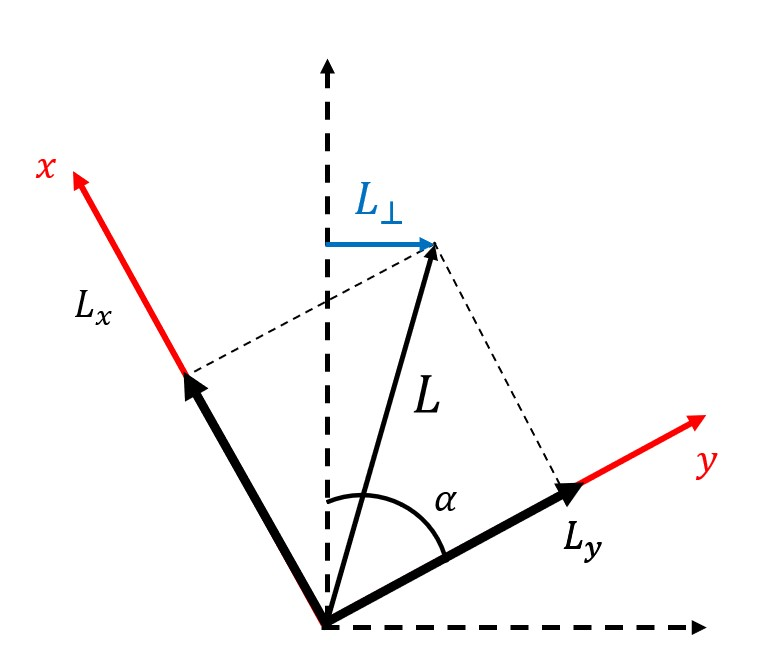
\includegraphics[scale=0.5]{diagram3.jpg}
    \caption{How I calculated torque}
    \label{3}
\end{figure}

\begin{equation}
    \begin{aligned}
        L_\perp & = L_y \sin\alpha- L_x \cos\alpha                                                                        \\
                & = (I_{1,y}\Omega +I_{2,y}\omega)\sin\alpha\cos\alpha-(I_{1,x}\Omega +I_{2,x}\omega)\sin\alpha\cos\alpha
    \end{aligned}
\end{equation}

Magnitude for rate of change of $L$ is
\begin{equation}
    \begin{aligned}
        \left|\frac{d\mathbf{L}}{dt} \right| & =\omega L_\perp                                                                              \\
                                             & = \omega\sin\alpha\cos\alpha ((I_{1,y}\Omega +I_{2,y}\omega)-(I_{1,x}\Omega +I_{2,x}\omega))
    \end{aligned}
\end{equation}

Expression for torque by gravity
\begin{equation}
    \tau_g = mg \ell\sin(\alpha-\beta)
\end{equation}
where $\ell=\sqrt{R_1^2+(d/2)^2}$ and $\beta=\arctan(d/2R_1)$


Equating torque to this expression gives us:
\begin{equation}
    mg \ell\sin(\alpha-\beta)=\omega\sin\alpha\cos\alpha ((I_{1,y}\Omega +I_{2,y}\omega)-(I_{1,x}\Omega +I_{2,x}\omega))
\end{equation}


\end{document}

